\documentclass[12pt]{extarticle}

%%%%%%% PACKAGES %%%%%%%%
\usepackage[utf8]{inputenc}
\usepackage[margin=2.5cm]{geometry}
\usepackage{blindtext}
\usepackage{setspace}
\usepackage{graphics}
%\usepackage{epstopdf}
\usepackage{notoccite} %citation number ordering
\usepackage{lscape} %landscape table
\usepackage{caption} %add a newline in the table caption
\usepackage{hyperref}
\usepackage{enumitem}
\usepackage{datetime}
\usepackage{titlesec}
\usepackage{booktabs} % For \toprule, \midrule and \bottomrule
\usepackage{siunitx} % Formats the units and values
\usepackage{pgfplotstable} % Generates table from .csv
\usepackage{amsmath}
\usepackage{bm}

\usepackage{chngcntr}
\counterwithin{figure}{section}
\titleformat*{\section}{\LARGE\bfseries}
\titleformat*{\subsection}{\Large\bfseries}
\titleformat*{\subsubsection}{\large\bfseries}

\newdateformat{monthyeardate}{%
	\monthname[\THEMONTH], \THEYEAR}

\onehalfspace   % 1.5 line spacing

\title{
\includegraphics[width=4cm]{pics/AAU_Logo.jpg}\\\Large{\textbf{Breast Cancer and Benign Detection using Hierarchical Deep Convolutional Neural Networks}}
\date{}}
\begin{document}
	\clearpage\maketitle
	\begin{center}
		\vspace{-1.5cm}
		\large{\emph{Submitted by}}\\\vspace{0.5cm}
		\begin{tabular}{l l}
			
			\multicolumn{1}{p{6cm}}{ \large{\textbf{Yacoub Abu Lubad}}} &  \multicolumn{1}{p{6cm}}{\centering \large{\textbf{201930007}}} 
		\end{tabular}\\\vspace{1cm}
		\large{\emph{Supervised by}}\\\vspace{0.5cm}
		\large{\textbf{Assistant Prof. Dr. Talal A. Edwan}}\\\vspace{1cm}
		{Submitted in partial fulfillment of the requirements for the award of the Bachelor of Science in Computer Engineering Degree\\\vspace{1cm}
		Faculty of Engineering\\Al-Ahliyya Amman University\\Amman - Jordan}\\ \vspace{0.5cm}
		\Large{\textbf{\monthyeardate\today}}
		\pagenumbering{roman} % Start roman numbering
		
		\thispagestyle{empty}
	\end{center}
	\newpage
	% % Start roman numbering
	\setcounter{page}{1}
	%%% CONTENT HERE %%%%
	\begin{center}
	\Large{\textbf{Acknowledgments}}\\ \vspace{1cm}
	\end{center}
	Acknowledgment Goes Here...
	\newpage
	
	\tableofcontents
	\listoffigures
	\listoftables
	\newpage
	\begin{center}
		\LARGE{\textbf{Abstract}}\\ \vspace{1cm}
	\end{center}
	Abstract goes here...\\
	Keywords: \emph{Keyword1, Keyword2, ... , Keywordn}
	\newpage
	\LARGE{\textbf{List of Abbreviations}}\\ \vspace{1cm}
	\begin{center}
		\begin{tabular}{l l}
			\multicolumn{1}{p{3cm}}{\large{\textbf{AI}}} &  \multicolumn{1}{p{8cm}}{\large{\textbf{A}rtificial \textbf{I}ntelligence}} \\
			\multicolumn{1}{p{3cm}}{\large{\textbf{ANN}}} &  \multicolumn{1}{p{8cm}}{\large{\textbf{A}rtificial \textbf{N}eural \textbf{N}etwork}} \\
			\multicolumn{1}{p{3cm}}{\large{\textbf{CNN}}} &  \multicolumn{1}{p{8cm}}{\large{\textbf{C}onvolutional \textbf{N}eural \textbf{N}etwork}}\\ 
			\multicolumn{1}{p{3cm}}{\large{\textbf{HD-CNN}}} &  \multicolumn{1}{p{8cm}}{\large{\textbf{H}ierarchical \textbf{D}eep \textbf{C}onvolutional \textbf{N}eural \textbf{N}etwork}}\\ 
			\multicolumn{1}{p{3cm}}{\large{\textbf{HDD}}} &  \multicolumn{1}{p{8cm}}{\large{\textbf{H}ard \textbf{D}isk \textbf{D}rive}}\\ 
			\multicolumn{1}{p{3cm}}{\large{\textbf{RAM}}} &  \multicolumn{1}{p{8cm}}{\large{\textbf{R}andom \textbf{A}ccess \textbf{M}emory}}\\ 
			\multicolumn{1}{p{3cm}}{\large{\textbf{CNN}}} &  \multicolumn{1}{p{8cm}}{\large{\textbf{C}onvolutional \textbf{N}eural \textbf{N}etwork}}\\ 
			\multicolumn{1}{p{3cm}}{\large{\textbf{CNN}}} &  \multicolumn{1}{p{8cm}}{\large{\textbf{C}onvolutional \textbf{N}eural \textbf{N}etwork}}
			 
		\end{tabular}
	\end{center}

	\newpage
	\LARGE{\textbf{List of Symbols}}\\ \vspace{1cm}
	\large{}
	\begin{center}
		\begin{tabular}{l l}
			{Symbol} & {Name} \\
			$b$ & bias\\
			$w$ & weights\\
			$\phi$ & activation function
		\end{tabular}
	\end{center}
	
	
	\newpage
	\large{}
	\pagenumbering{arabic}
	\section{Introduction}
	The \emph{motivation} of this Thesis will be discussed in Section \ref{Motiv}, while explaining more what the \emph{actual problem} is and the \emph{purpose of this Thesis} in Section \ref{delay problem}. As for the \emph{objectives} of this Thesis, that will be briefly discussed in Section \ref{Obj}, while the \emph{organization} and the structure of this Thesis is to be discussed in Section \ref{Org}.
	\subsection{Motivation}\label{Motiv}
	
	Breast cancer is the most common cause of new cancer cases, according to the \textbf{World Health Organization (WHO)}, standing at 2.26 million recorded cases in 2020, meanwhile, the total count of cancer caused mortality cases are recorded to be 10 million in 2020, breast cancer is documented to have caused 685,000 deaths in 2020 \cite{WHO_stats}. There are multiple ways of reducing the mortality rate of this disease, one of the main approaches would be early detection. A study has proved that a delayed diagnosis and detection of \emph{more than 6 weeks} gave these cancerous cells enough time to develop into much dangerous stages, but diagnosis that were conducted \emph{under 6 weeks} of delay detected less advanced stages of these cells \cite{caplan2014delay}. So the earlier the detection of these cells are prompted, the safer and less severe it is on the patient.
	\\[5mm]
	This sort of detection is done via Screening Mammography where a patient undergoes 4 different kinds x-ray imaging, one image is taken from the side of the breast and the second is from the top, same procedure is repeated on the second breast \cite{healthline}. This totals in 4 images per patient where the radiologist can evaluate whether there are any \emph{abnormalities} detected, which are usually \emph{lumps} that are classified into two categories, \emph{Benign and Cancer}. The only downfall is that if any abnormalities are detecting after the first evaluation, the patient is contacted, which could typically take up to a week or two, to visit and perform a diagnostics test so that the abnormality could be studied even further in classifying whether it is cancerous or not \cite{healthline}.\\[5mm]
	
	\subsubsection{The result delay problem}\label{delay problem}
	As discussed in Section~\ref{Motiv}, the issues of late diagnosis and detection of these cancerous cells would increase the mortality rate, and it has also been pointed out that the results of any abnormalities detected by the radiologist could only be known after a duration of week or two. This problem can be tackled by reducing the time of detecting the abnormalities from \emph{1-2 weeks} all the way down to matter of \textbf{fractions of a second.}\\[5mm]
	This method is a great aid in early detection, this way the patient would have a time advantage to proceed to the diagnosis of this abnormality right away. However, it is also possible to \emph{skip} the diagnosis procedure as well, saving even more time when all it would require is one mammography screening and the results would be ready the moment the screening is completed.\\[5mm]
	A key feature in making this quick and accurate detection is using two methods that fall under the \textbf{Artificial Intelligence (AI)} domain, \emph{Image Classification} and \emph{Object Detection}.
	
	\subsection{Objectives}\label{Obj}
	The goal of this thesis is to compare and contrast the different results that could be obtained using different \emph{Convolutional Neural Network} (CNN) model structures. Applying \textbf{4 different concepts} to the same dataset but with different utilization of the data to measure the accuracy that might be obtained when manipulating the data differently. Due to the vast dataset that was obtained, one of the multiple hardware constraints were during loading the images from the \emph{Hard Disk Drive} (HDD) onto the \emph{Random Access Memory} (RAM), there was no enough memory to load the whole dataset to proceed with the model training. \\[5mm]
	A different kind of hardware constraint that was faced is the absence of \emph{Graphical Processing Unit} (GPU), a GPU is crucial for \emph{Computer Vision} (CV) due to the enormous data stream that will take place during training \cite{GPU}.
	\subsection{Organization}\label{Org}
	The \emph{Literature Review} will be discussed in \emph{Section~\ref{Lit. Rev.}} alongside the essential background on the different kinds of Neural Networks with their diverse functionalities. A deeper dive into the application's functions will be thoroughly described in \emph{Section~\ref{CV}} and the two main techniques that will be implemented in this Thesis. In \emph{Section~\ref{Meth}}, there will be a detailed explanation on the \textbf{Hierarchical approach} that is applied to obtain the results as well as the methods that helped surpassed the constraints that were mentioned in \emph{Secion~\ref{Obj}}. Detailed dissection of the dataset will be in \emph{Section~\ref{Data}}.
	\newpage
	\section{Background}\label{Lit. Rev.}
	Lit. Rev. goes here
	\subsection{Artificial Neural Networks}\label{ANN}
	\emph{Artificial Neural Networks} (ANN) are a simplified mathematical models that mimic the functionality of a human brain and nervous system \cite{ANN, ANN2}. Just like humans, these networks were designed to solve more complex, \emph{non-linear}, highly stochastic and multi-variable problems that a traditional program could not. These problems span out to the fields of medicine, finance, security and many more \cite{ANN_funct}. \emph{ANNs} are designed to approximating any continuous function thus are used in a wide spectrum of applications such as object detection \cite{Objdet, Objdet2}, image classification \cite{classification}, image enhancement \cite{enhancement} as well as several more uses.\\[5mm]
	The \emph{ANN} is originally compromised from multiple \emph{neurons}, or \emph{perceptron}, which can be demonstrated in \emph{Figure~\ref{fig:Perceptron}}, hence the \emph{perceptron} is the ground foundation of \emph{ANNs}.
	\begin{figure}[h]
		\centering
		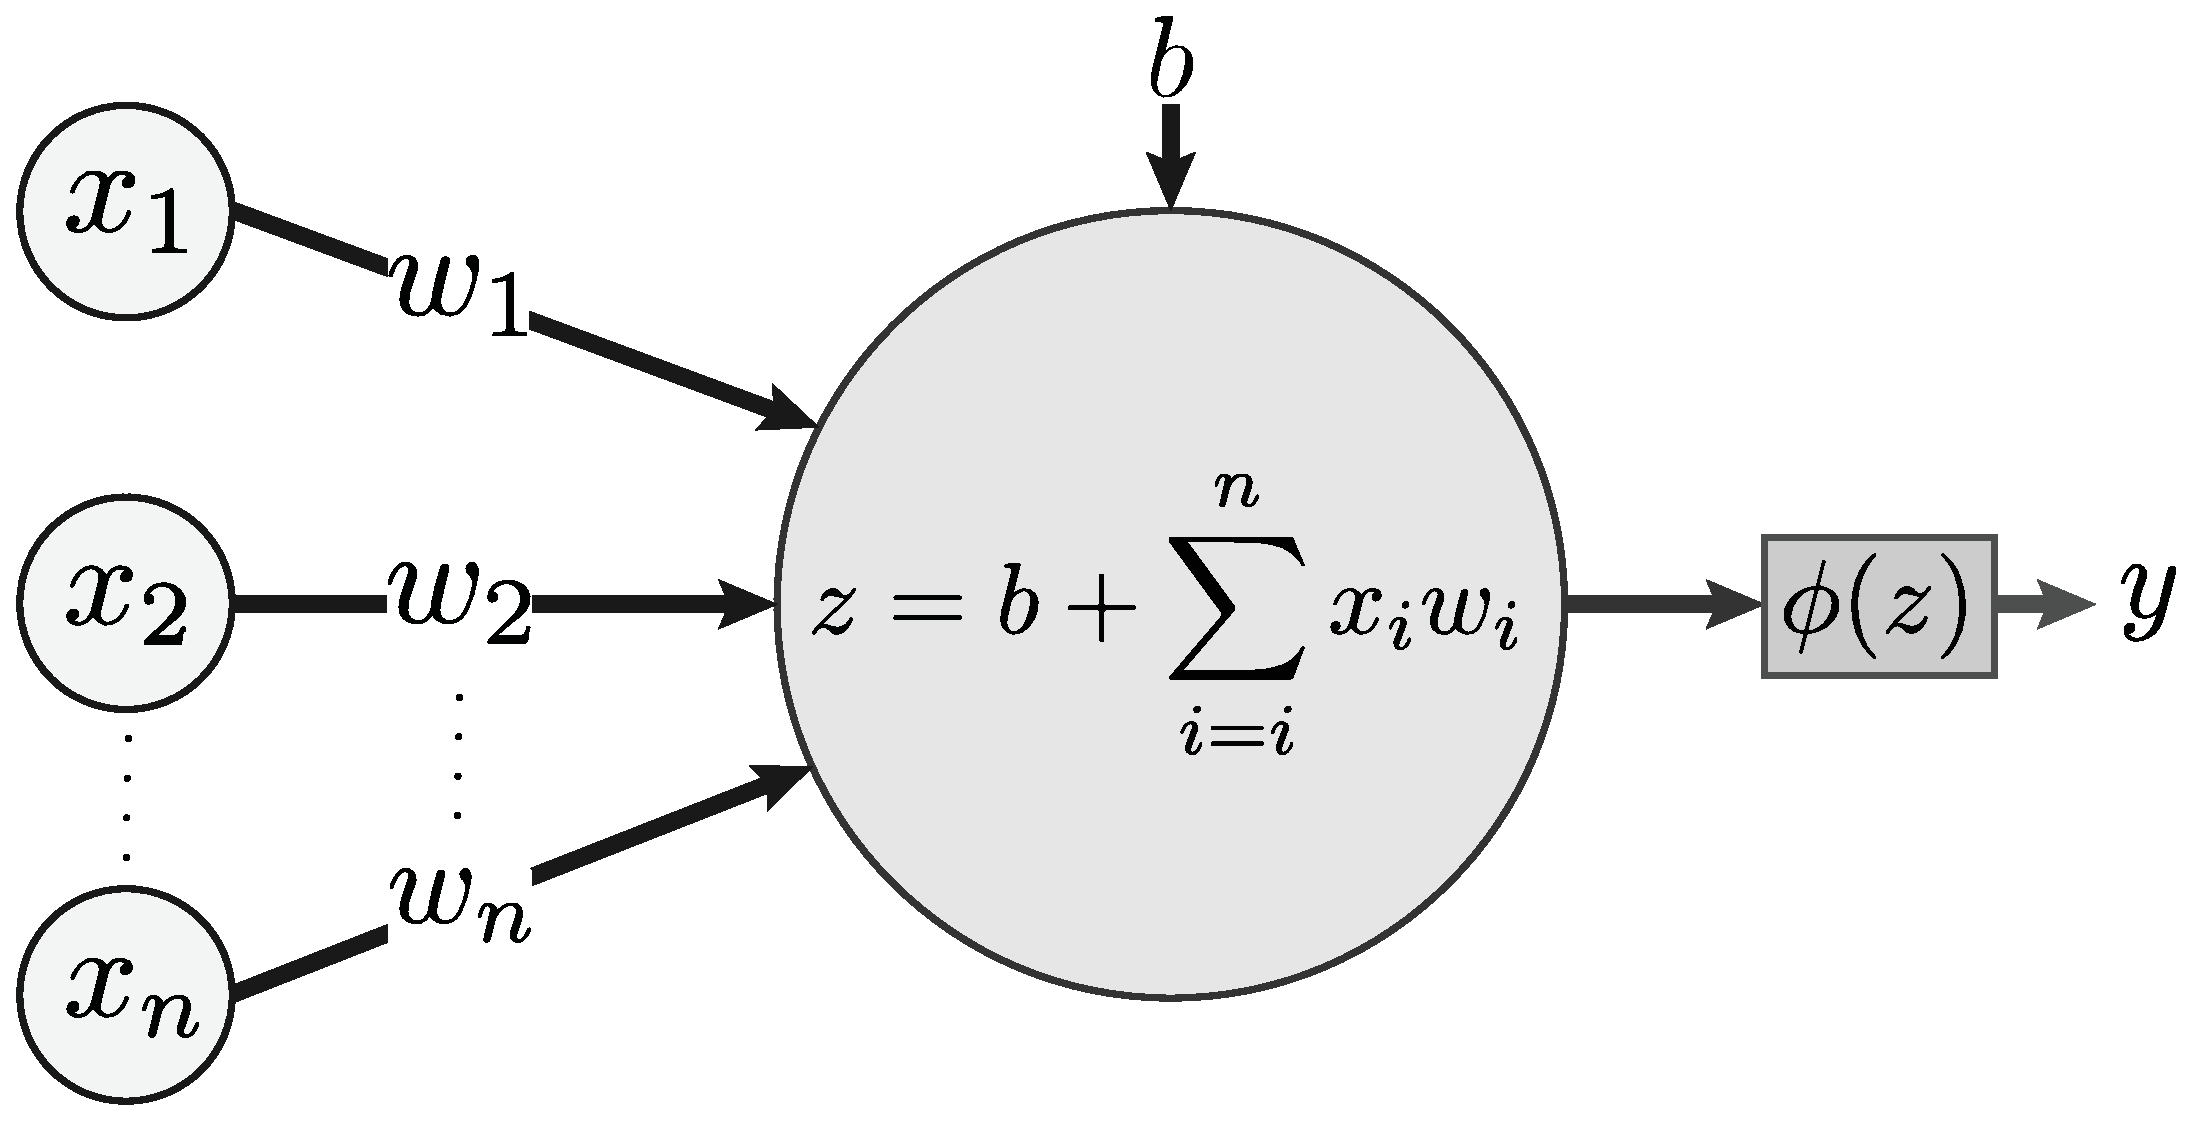
\includegraphics[width=0.7\textwidth]{pics/Figures/Perceptron.eps}
		\caption{\small{Artificial Neuron \emph{(Perceptron)}}}
		\label{fig:Perceptron}
	\end{figure}
	
	The input $\bm{x}$ of size $\bm{n}$ for this perceptron is denoted as the input vector that is composed of numerical values representing different features of a single entry as seen below.
	\begin{align}
	x &= \begin{bmatrix}\label{inputs}
		x_1 \\
		x_2 \\
		\vdots \\
		x_n
	\end{bmatrix}
	\end{align}

	Depending on the features of a given model data, different features require different \emph{weights}, denoted as $\bm{w}$, since one feature would have more effect on the final output more than a different kind of feature, thus an input must be multiplied with a weight to determine its importance to the final output.\\
	\begin{align}
		w &= \begin{bmatrix}\label{weights}
			w_1 \quad
			w_2 \quad
			\cdots \quad
			w_n
		\end{bmatrix}
	\end{align}
	
	The above vector will differ based on the next layer's size, given that there is $\bm{m}$ number of neurons in the next layer, the \emph{weight's matrix} will have a size of $\bm{m \times n}$ as seen in \emph{Equation~\ref{weights_expanded}}. The weight vector is a \emph{row vector} due to the relationship it contains with the input as every $\bm{n^{th}}$ input, there's a $\bm{n^{th}}$ weight corresponding to it.\\[5mm]
	After the input is multiplied with its assigned weight, it is now referred to as the \textbf{weighted input}, that weighted input is summed with the rest of the weighted inputs which then derives us the \textbf{weighted sum}. Then as all these inputs are summed, a \emph{bias} $\bm{b}$ is added which is an additional parameter that is used to adjust the \emph{output} of the perceptron as well as the weighted sum that is \emph{inputted} into the perceptron.\\[5mm]
	\newpage
	The output of the perceptron can be denoted as $\bm{y}$ and is calculated as follows:
	\begin{equation}\label{output}
		y = \phi{(z)},
	\end{equation}
	where
	\begin{equation}\label{z}
		z = b + \sum_{i}^{n} x_i w_i
	\end{equation}
	
	The $\bm{\phi}$ is an arbitrary function known as the \textbf{activation function} which is responsible for causing the perceptron to \emph{fire} generating an output. This activation function is deduced by a threshold that is set based on the different types of activation functions alongside their different uses which can limit the output of reaching an undesired or unacceptable value \cite{siddique2013computational}.\\[5mm]
	
	The expansion from a single perceptron to multi perceptrons forms a \emph{single layered neural network} as seen in \emph{Figure~\ref{fig:ANN}}; using the input vector as seen in \emph{Equation \ref{inputs}} and defining the weights matrix 
	\begin{align}
		 w &= \begin{bmatrix}\label{weights_expanded}
			w_{1,1}\quad w_{1,2} \quad \cdots \quad w_{1,n}\\
			w_{2,1} \quad w_{2,2} \quad \cdots \quad w_{2,n}\\
			\vdots \qquad \vdots \qquad \ddots \qquad \vdots\\
			w_{m,1} \quad w_{m,2} \quad \cdots \quad w_{m,n}
		\end{bmatrix}
	\end{align}
	where $\bm{m}$ is the number of perceptrons and $\bm{n}$ is the number of inputs
	\begin{figure}[h]
		\centering
		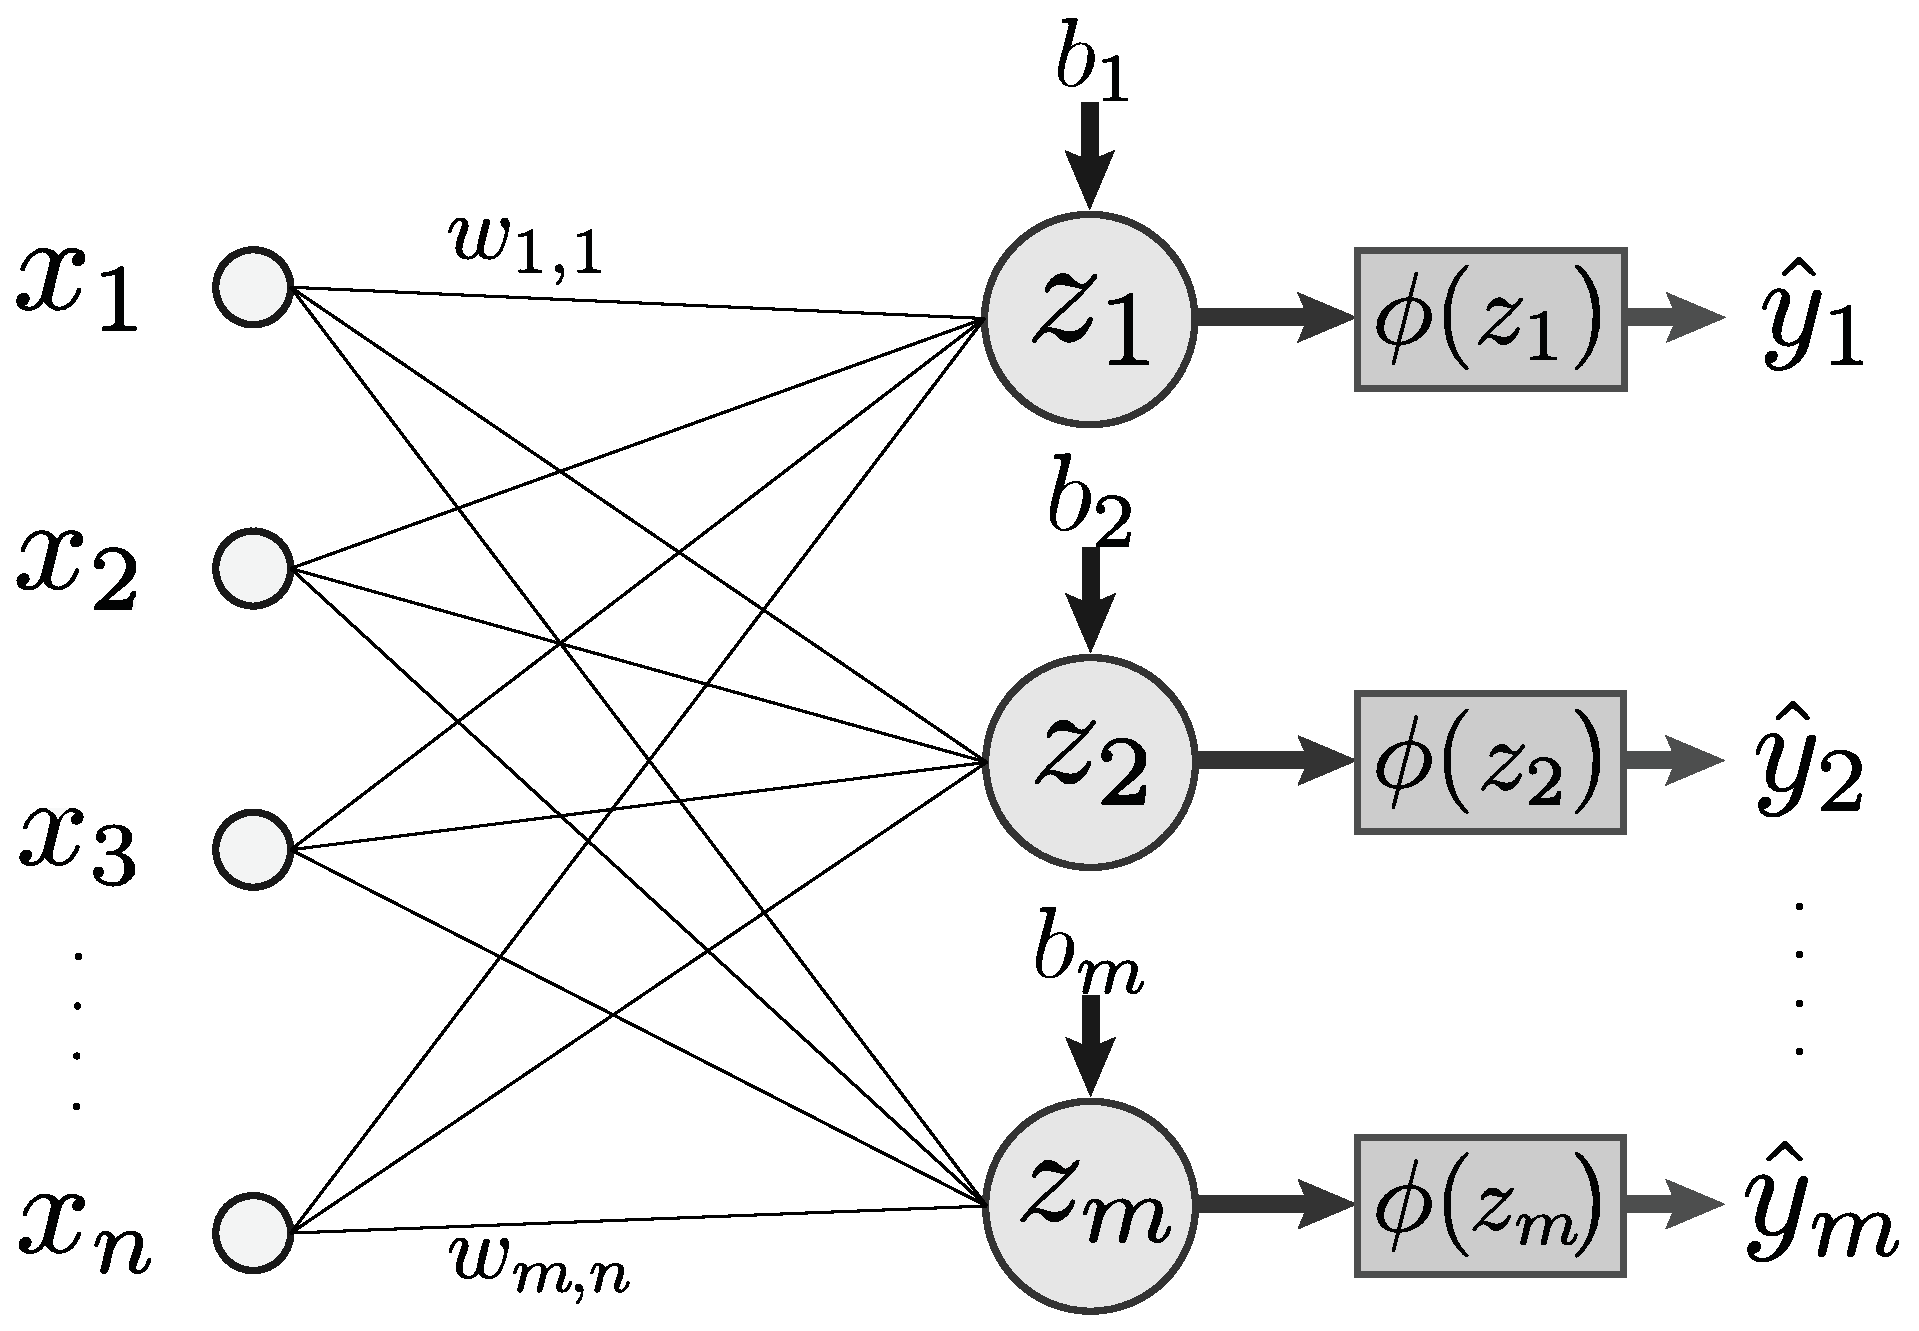
\includegraphics[width=0.7\textwidth]{pics/Figures/ANN.eps}
		\caption{\small{Artificial Neural Network Model \emph{(Single Layer)}}}
		\label{fig:ANN}
	\end{figure}
	
	\subsubsection{Multi Layer Perceptron}\label{MLP}
	Some text about \emph{Multi Layer Perceptron} (MLP)
	
	
	\subsubsection{Convolutional Neural Networks}\label{CNN}	
	Some text about \textbf{Convolutional Neural Networks (CNN)}
	\subsection{Computer Vision}\label{CV}
	Some text about \textbf{Computer Vision (CV)}
	\subsubsection{Image Classification}\label{Classification}
	Some text about \textbf{Image Classification}
	\begin{figure}[h]
		\centering
		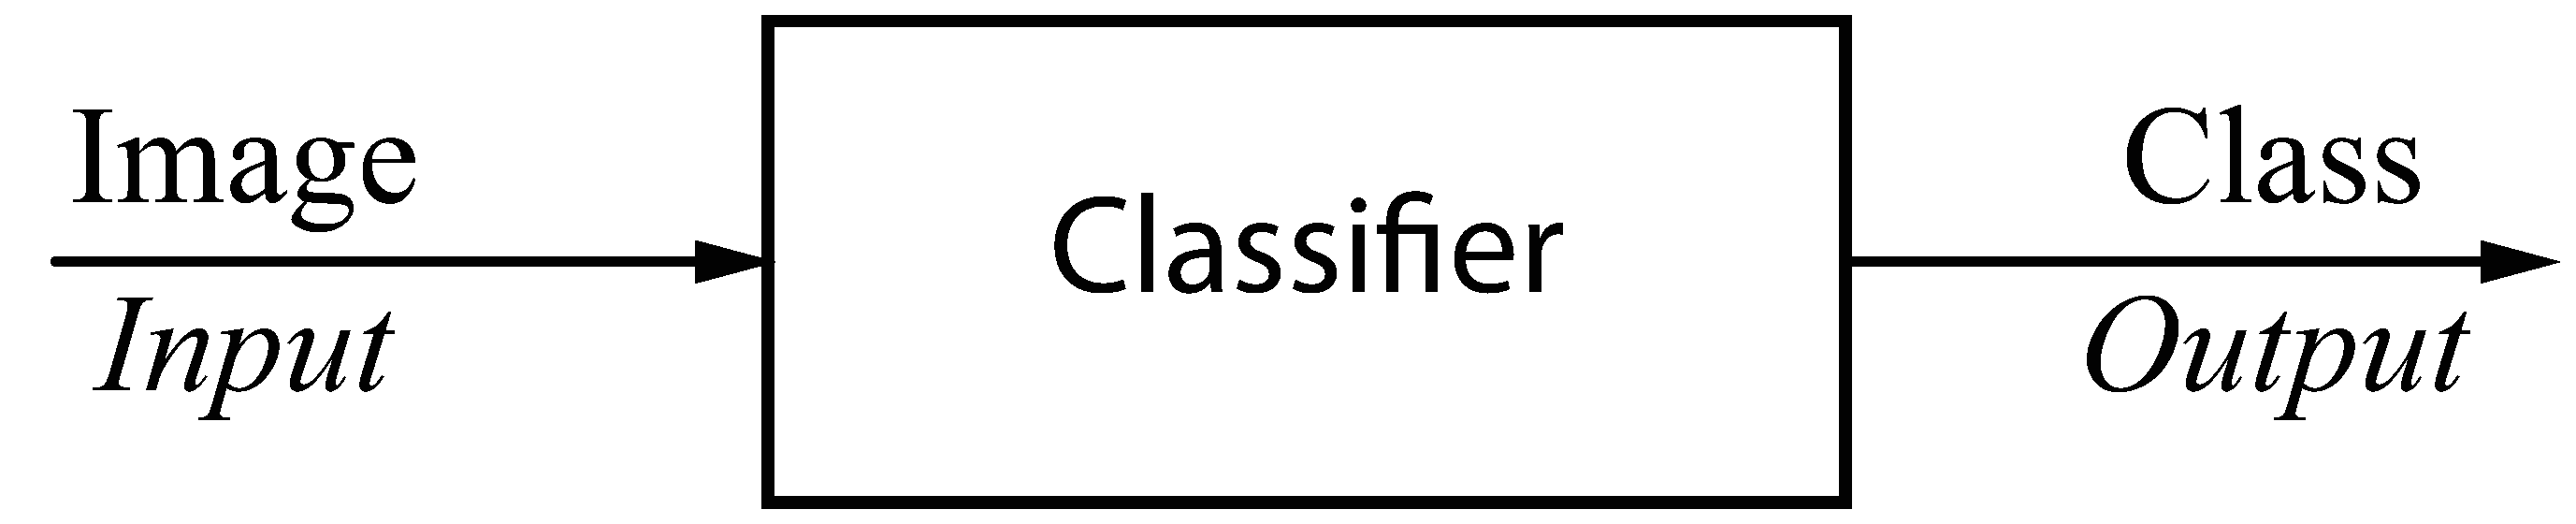
\includegraphics[width=0.5\textwidth]{pics/Figures/Classifier_Block_Diagram.eps}
		\caption{\small{Classifier Diagram}}
		\label{fig:Classifier}
	\end{figure}
	\subsubsection{Object Detection}\label{Obj Detection}
	Some text about \textbf{Object Detection}\\
	\begin{figure}[h]
		\centering
		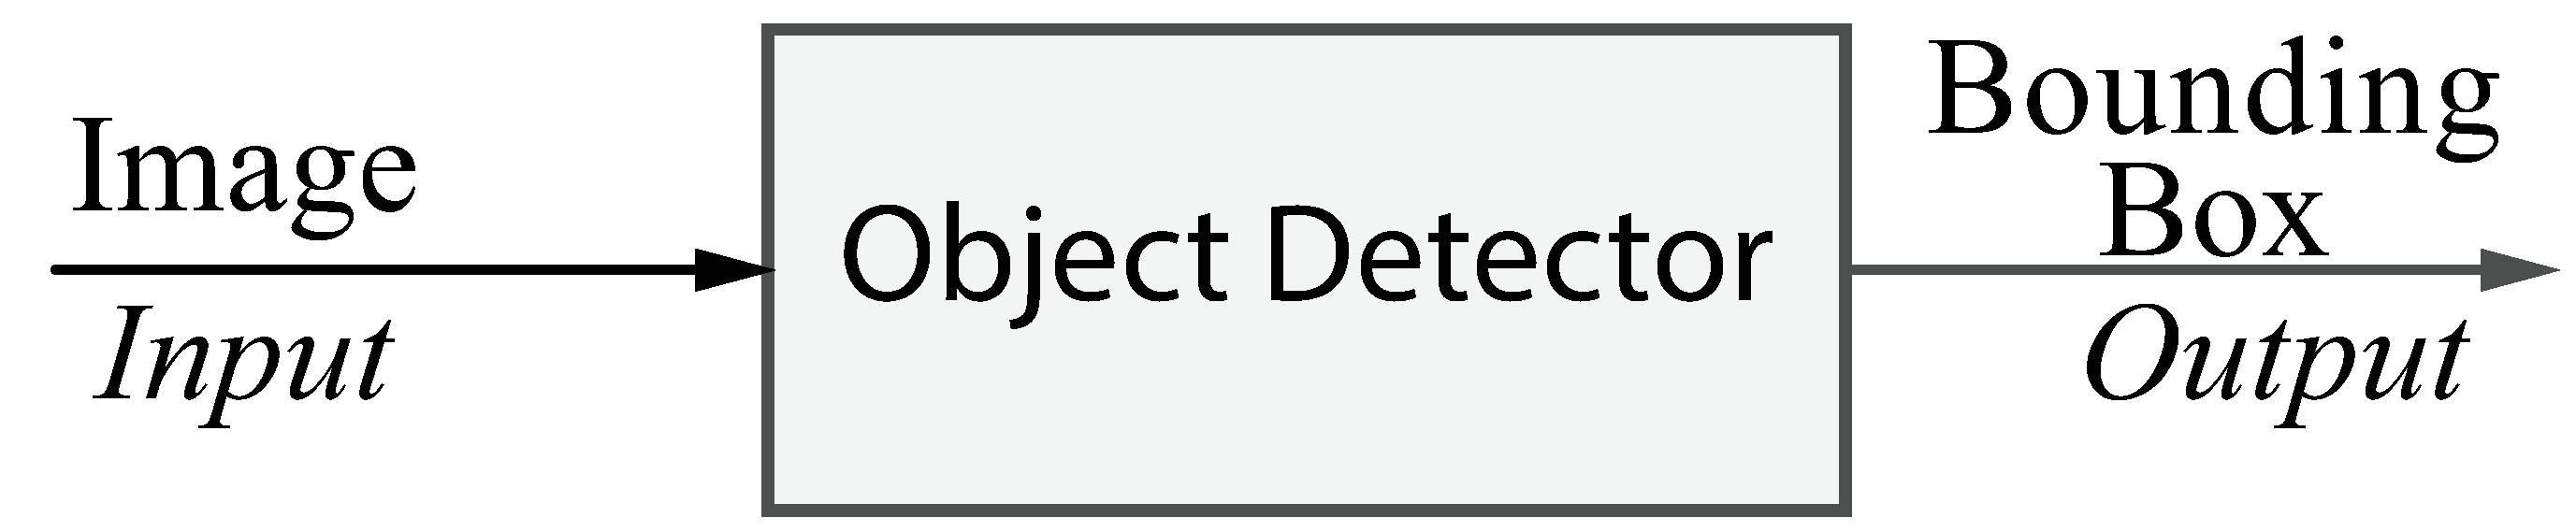
\includegraphics[width=0.5\textwidth]{pics/Figures/Obj_Det_Block_Diagram.eps}
		\caption{\small{Object Detection Diagram}}
		\label{fig:Obj Detector}
	\end{figure}
	
	\subsection{Hierarchy Classifier}
	An explanation on the Hierarchical approach.
	\begin{figure}[h]
		\centering
		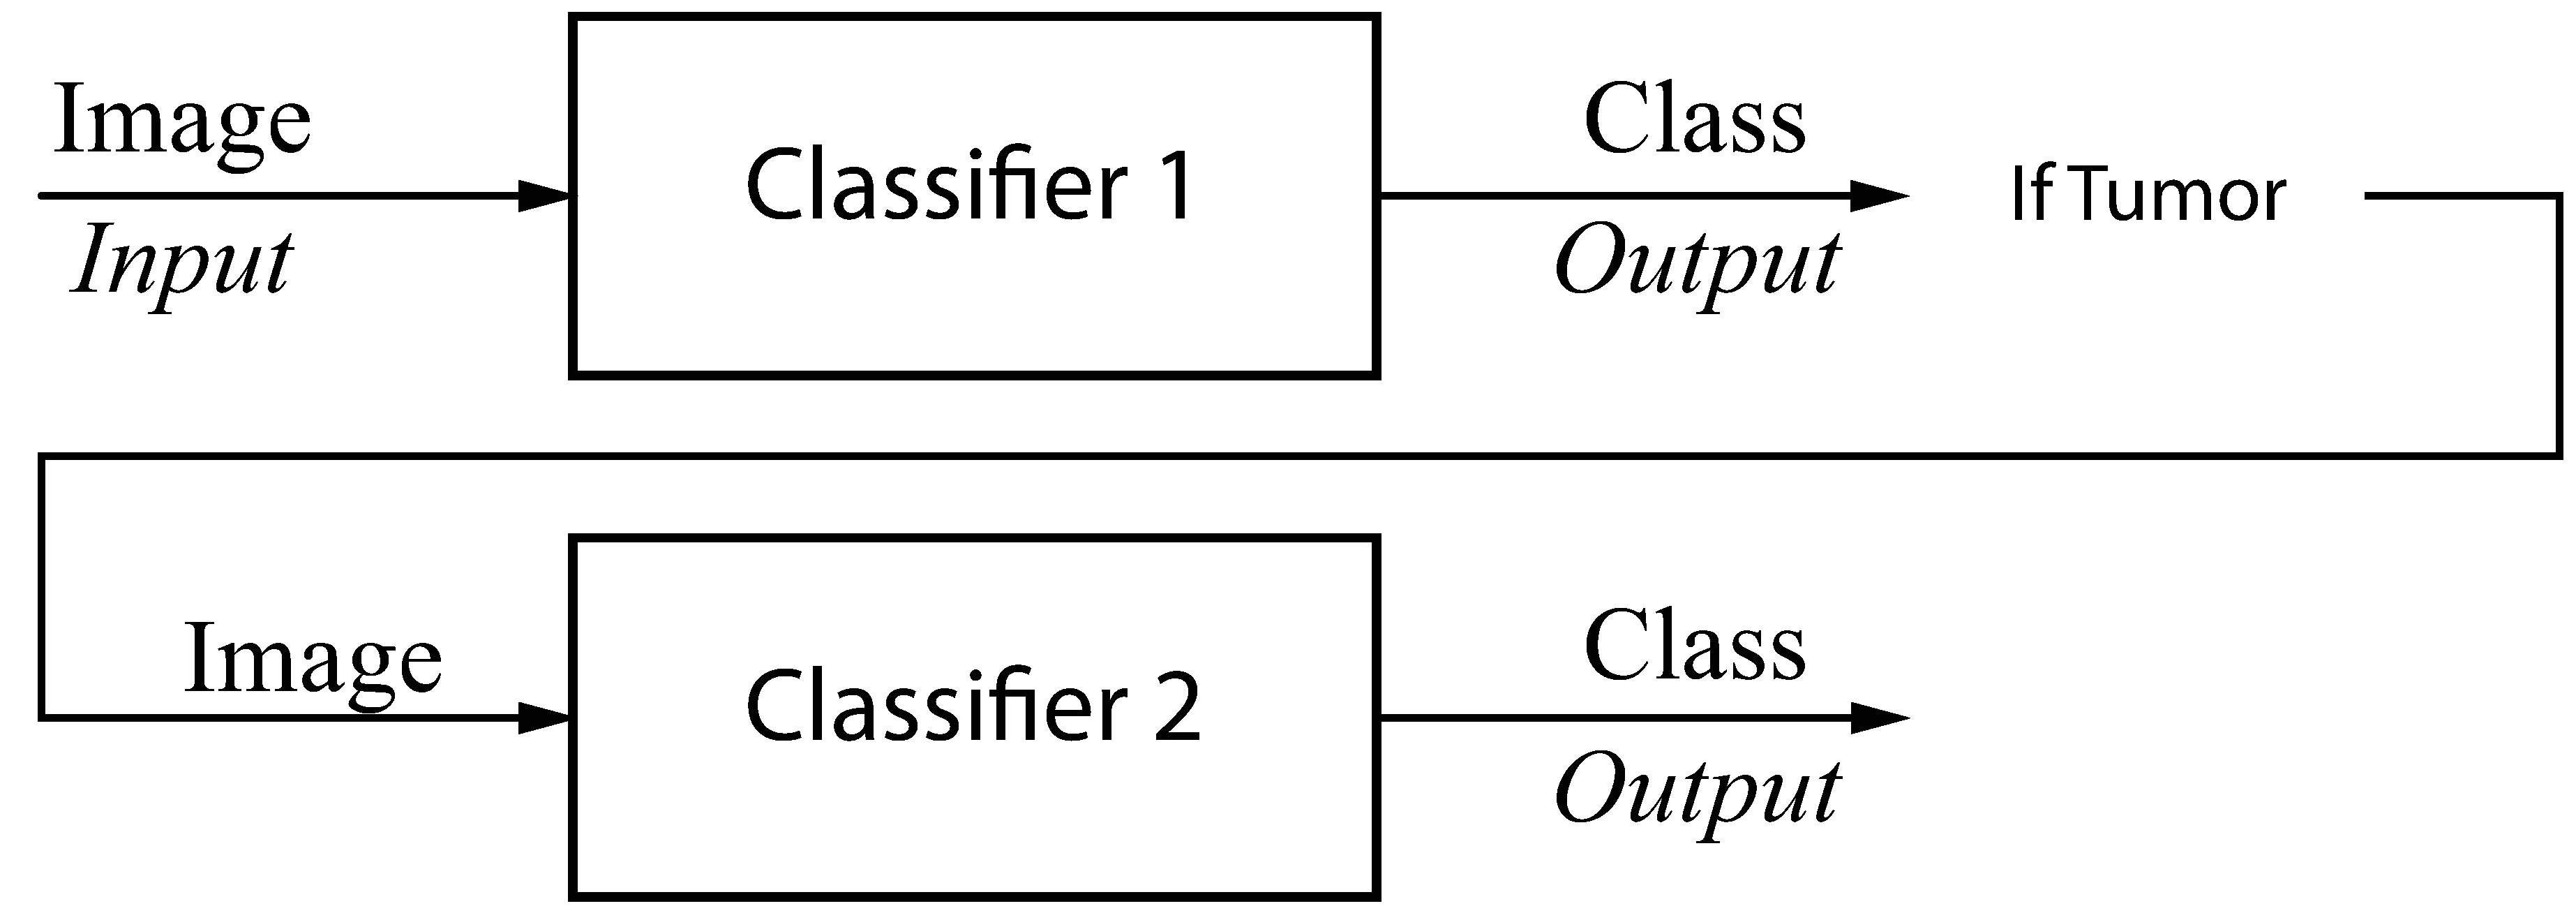
\includegraphics[width=0.5\textwidth]{pics/Figures/Hierarchical_Classifier_Block_Diagram.eps}
		\caption{\small{Hierarchical Classifier Diagram}}
		\label{fig:Hierarchical Classifier}
	\end{figure}
	some basic explanation on \emph{Figure \ref{fig:Hierarchical Classifier}} which is a normal approach found in /ref{GJU paper}.
	\newpage
	
	
	\section{Hierarchical Method}\label{Meth}
	
	\begin{figure}[h]
		\centering
		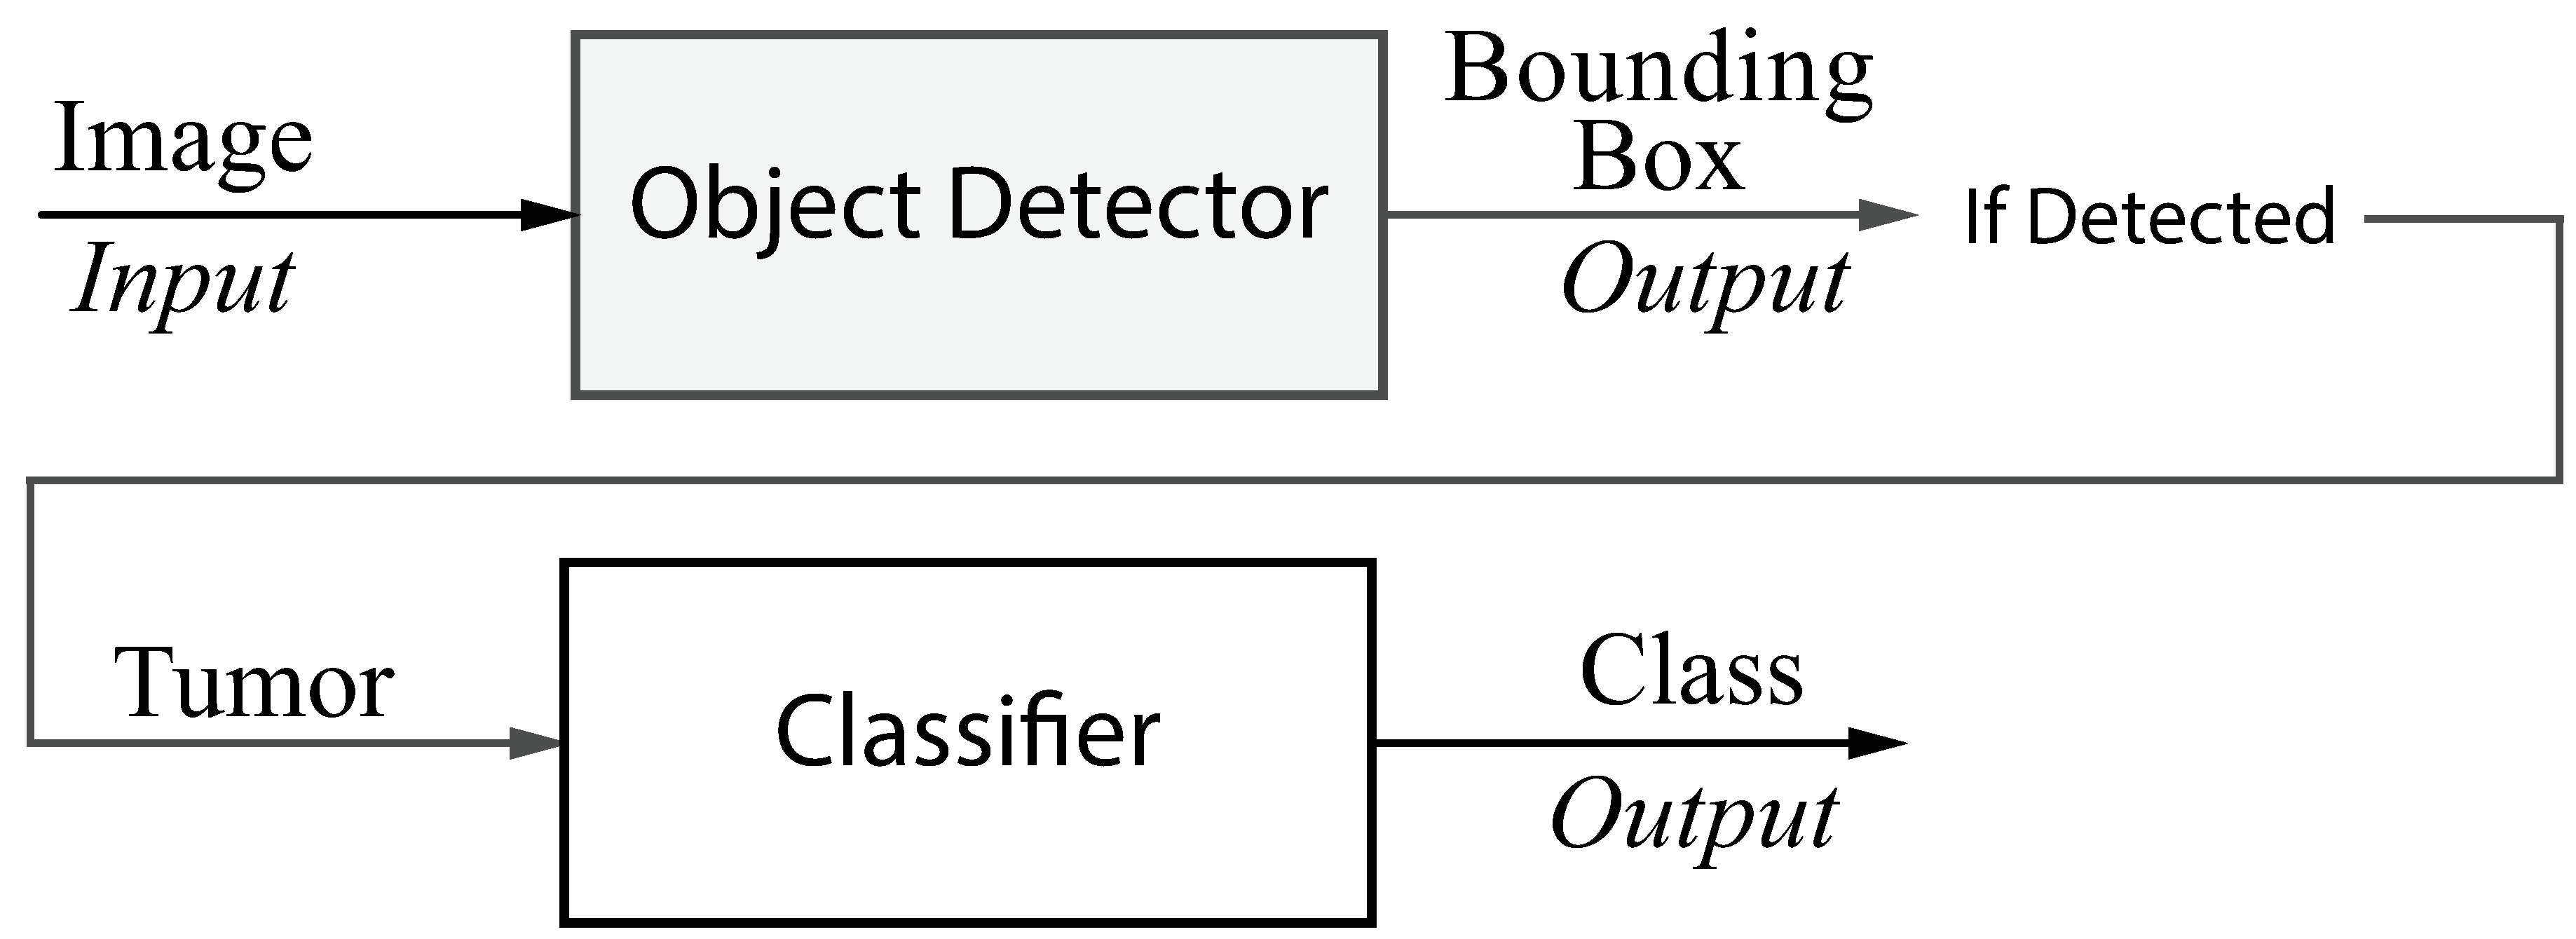
\includegraphics[width=0.5\textwidth]{pics/Figures/Hierarchical_Obj_Det_Block_Diagram.eps}
		\caption{\small{Object Detection Diagram}}
		\label{fig:Hierarchical Obj Detector}
	\end{figure}
	some in depth explanation on \emph{Figure \ref{fig:Hierarchical Obj Detector}} alongside many more figures to explain the thought process 
	\subsection{Dataset}\label{Data}
	
	Choosing a dataset for this problem is crucial to many stages, first and foremost is the \emph{quality of the data}. Does the data clearly portray the goal that should be acquired? Secondly is the \emph{quantity of the dataset}, just like the quality, quantity is as important. \textbf{Neural Networks} require a lot of data, but the quantity mainly depends on the following:
	\begin{itemize}
		\item features that must be extracted from the data
		\item type of Neural Network
		\item data quality
		\item the desired goal
	\end{itemize}
	With that being said, the data is a vital part of this project, and to be able to achieve high accuracy and precision of detecting the cancerous cells, it is a must to obtain high grade dataset. 
	The most common age for the diagnosis of breast cancer is \emph{over 50} years of age. This has been conducted by the National Cancer Institute that the median age of breast cancer patients is between the age of \emph{55} to \emph{64} \cite{CDC}. 
	\\[5mm]
	
	
	\begin{figure}[h]
		\centering
		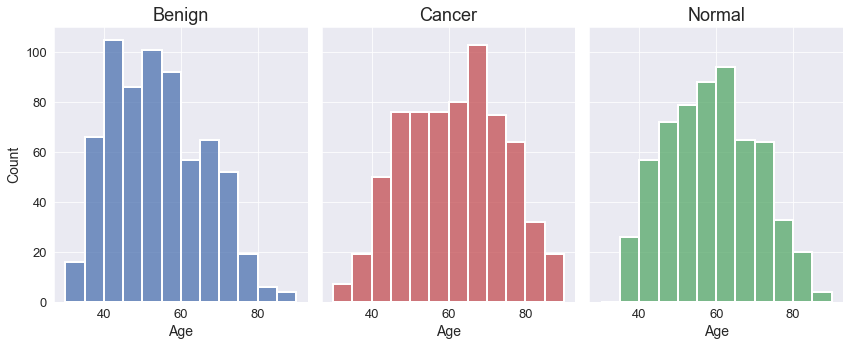
\includegraphics[width=1\textwidth]{pics/Figures/Age_Dist.png}
		\caption{\small{Age Distribution}}
		\label{fig:Age_Dist}
	\end{figure}
	\begin{figure}[h]
		\centering
		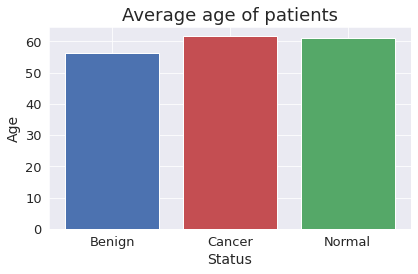
\includegraphics[width=0.5\textwidth]{pics/Figures/Avg_Age.png}
		\caption{\small{Average Age}}
		\label{fig:Avg_Age}
	\end{figure}
	
	\newpage	
	\section{Conclusion}
	Conclusion goes here
	\newpage

	\bibliographystyle{IEEEtran}
	\bibliography{IEEEabrv,myrefs}
	
	
\end{document}

\newpage
\setstretch{1}  %reduce bibliography line spacing
\end{document}